\chapter{Approccio proposto}%\label{ch:chapter1}

L'approccio che \`e stato utilizzato si articola in pi\`u fasi che andremo a vedere nel corso di questo capitolo.

\section{Preprocessing}

Le immagini di partenza sono lette e convertite in immagini in scala di grigi usando \emph{OpenCV} (gli scan di partenza sono a colori).

Successivamente vengono binarizzate, ovvero passano da essere in scala di grigi ad essere in bianco e nero. Per la binarizzazione viene usata la soglia di 128, quindi tutti i pixel che hanno un valore $<128$ diventano neri, mentre quelli con un valore $\ge128$ diventano bianchi.

Il valore di soglia (128), pu\`o chiaramente essere cambiato. \`E stato scelto il valore di 128 poich\'e a met\`a fra 0 e 255, che \`e il massimo valore che pu\`o avere un pixel in scala di grigi nella risoluzione a 8 bit per ogni pixel. Inoltre il valore di 128 sembra funzionare bene per le immagini di nostro interesse.

Se si dovessero analizzare altri scan, si pu\`o aggiustare il valore di soglia o addirittura cambiare il metodo di binarizzazione usandone uno pi\`u raffinato.

\section{Segmentazione}\label{sect:segmentation}

Per segmentazione si intende la separazione del documento nei vari caratteri che lo compongono. Questo processo non pu\`o essere perfetto se non si conosce la lingua che si vuole leggere, poich\'e in certi casi nella scrittura a mano possono esserci dei tratti ambigui che si riescono a capire solamente guardando il contesto della parola o addirittura della frase.

\subsection{Separazione delle righe}

Prima di separare i caratteri di una parola dobbiamo separare il documento nelle righe di testo che lo compongono. Per fare ci\`o, possiamo contare, in ciascuna riga di pixel, quanti sono neri e prendere i minimi relativi come punti di separazione. Nella figura \ref{fig:horiz_proj} \`e riportato il grafico del numero di pixel neri delle righe in una pagina.

\begin{figure}
%    \centering
    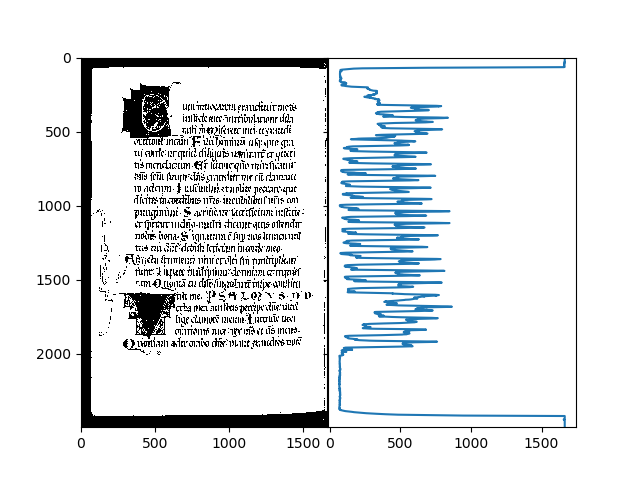
\includegraphics[width=\textwidth]{figures/horizontal-projection.png}
    \caption{A sinistra l'immagine binarizzata, a destra il conto dei pixel neri in ciascuna riga dell'immagine (sulle ordinate il numero della riga e sulle ascisse il numero di pixel).}
    \label{fig:horiz_proj}
\end{figure}

Guardando attentamente la figura \ref{fig:horiz_proj}, si nota che i minimi relativi del grafico sono molti di pi\`u delle righe di testo e, in particolare, molti minimi vanno a cascare nel mezzo di una riga. Questo \`e un problema che possiamo risolvere con delle finestre scorrevoli.

\subsubsection{Media mobile}

Per calcolare la media mobile possiamo utilizzare una finestra scorrevole. Applicare una finestra scorrevole di grandezza $n$ ad un array di numeri, significa sostituire ad ogni valore, la media degli $n$ valori pi\`u vicini. Questo processo tende a far diminuire la differenza fra un elemento e il successivo e porta ad eliminare molti massimi e minimi relativi.

Nella figura \ref{fig:all_smooth} possiamo vedere come la finestra scorrevole agisce sull'array di partenza. In particolare in figura \ref{fig:horiz_proj_smooth} possiamo vedere come i minimi relativi adesso si trovano sempre fra due righe di testo.

\begin{figure}
    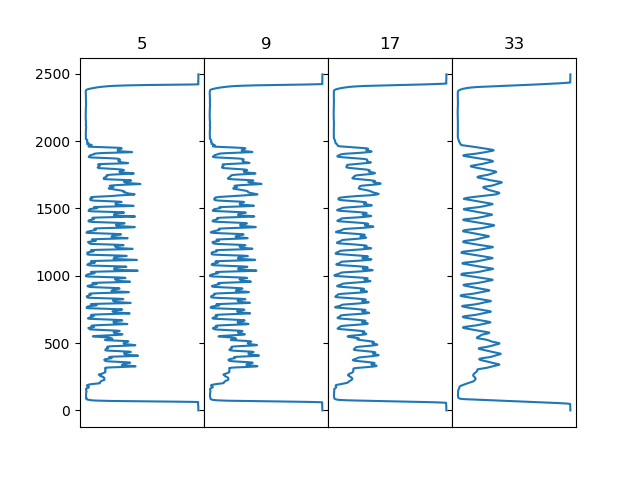
\includegraphics[width=\textwidth]{figures/all-smooth.png}
    \caption{I grafici relativi a finestre scorrevoli di varia grandezza (sopra ciascun grafico \`e segnata la dimensione della finestra).}
    \label{fig:all_smooth}
\end{figure}

\begin{figure}
    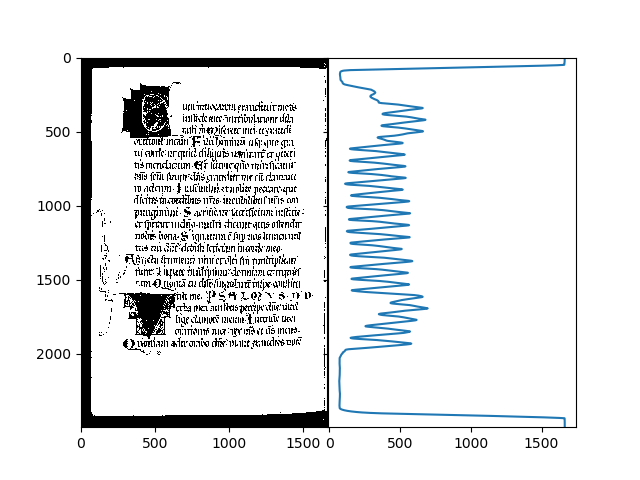
\includegraphics[width=\textwidth]{figures/horizontal-projection-smoothed.png}
    \caption{L'immagine di partenza affiancata alla proiezione a cui \`e stata applicata una finestra scorrevole di 33.}
    \label{fig:horiz_proj_smooth}
\end{figure}

\subsection{Separazione dei caratteri}

Nonostante non si possa sperare di separare i caratteri con esattezza, possiamo comunque separare le varie righe e fare delle ipotesi sui punti in cui finisce un carattere e inizia il successivo usando lo stesso metodo visto per separare le righe.

In figura \ref{fig:vert_proj_smooth} si vede una riga di testo e la proiezione verticale corrispondente ad una finestra scorrevole di dimensione 9; mentre nella figura \ref{fig:sectioned_row} \`e presente la stessa riga con delle barre verticali in corrispondenza dei minimi relativi.

\begin{figure}
    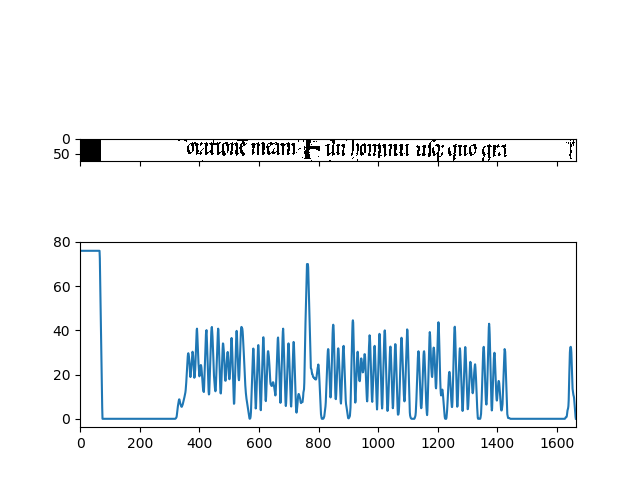
\includegraphics[width=\textwidth]{figures/vertical-projection-smooth.png}
    \caption{Sopra la riga di testo e sotto il grafico della proiezione verticale a cui \`e stata applicata una finestra scorrevole di dimensione 9.}
    \label{fig:vert_proj_smooth}
\end{figure}

\begin{figure}
    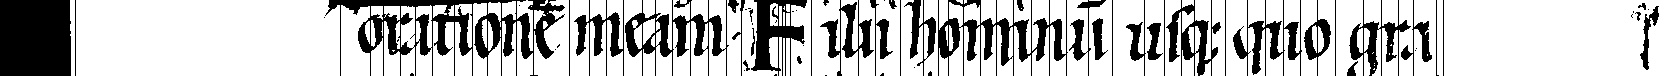
\includegraphics[width=\textwidth]{figures/Bodmer 30_012v_large.jpg_sectioned_row_10.jpg}
    \caption{Una riga di testo sezionata verticalmente.}
    \label{fig:sectioned_row}
\end{figure}

Come si vede dalla figura \ref{fig:sectioned_row} e come avevamo predetto all'inizio del capitolo, la separazione dei caratteri non \`e stata perfetta. Nonostante ci\`o, i corretti punti di divisione sono tutti stati individuati, l'unico problema \`e che sono stati individuati anche punti di divisione incorretti. Questo non sar\`a comunque un problema come vedremo nel capitolo successivo.

\section{Estrazione delle lettere}

Per estrarre le lettere da una riga di testo come quella in figura \ref{fig:sectioned_row}, dobbiamo guardare non solo i rettangoli di pixel che sono delimitati da due minimi nella proiezione verticale, ma dobbiamo anche guardare gruppi di 2 o 3 rettangoli contigui. Molte lettere, infatti, sono separate da 1 linea verticale e alcune, come la \emph{m}, anche da 2.

Adesso che abbiamo una porzione di immagine rettangolare come quella in figura \ref{fig:unpolished_letter}, dobbiamo estrarre la lettera vera e propria. Infatti, si possono vedere dei pezzi delle lettere confinanti che sono entrati nel rettangolo corrispondente alla nostra lettera.

\begin{figure}
    \centering
    \frame{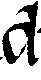
\includegraphics{figures/Bodmer 30_012v_large.jpgstaticd1.png(7, 56, 2).png}}
    \caption{Un rettangolo dell'immagine contenente la lettera \emph{d}.}
    \label{fig:unpolished_letter}
\end{figure}

\subsection{Componenti connesse}

Per prima cosa dobbiamo individuare le componenti connesse dell'immagine. Consideriamo un grafo non orientato che ha come vertici i pixel neri e come archi quelli andiamo adesso a definire. Possiamo dire che esiste un arco fra due vertici, se i pixel (poligoni) corrispondenti condividono un lato (connessione a 4) oppure se condividono un lato o un vertice (connessione a 8). La figura \ref{fig:connectivity} mostra i due diversi tipi di connessione.

\begin{figure}
    \centering
    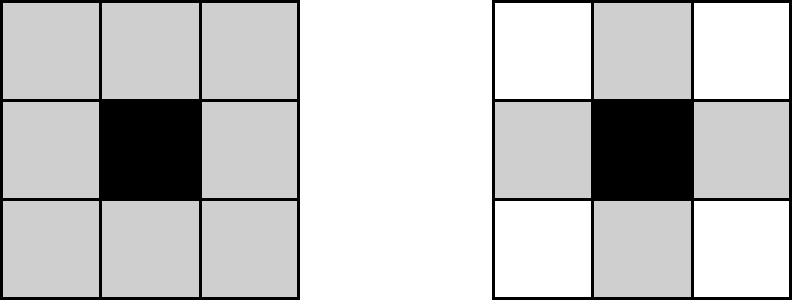
\includegraphics[width=0.5\textwidth]{figures/Sasiedztwa_4_8.png}
    \caption{I due tipi di connessione. A destra la connessione a 4 e a sinistra la connessione a 8.}
    \label{fig:connectivity}
\end{figure}

Nel nostro caso utilizzeremo la connessione a 4, ma dobbiamo tenere a mente che abbiamo sempre l'opzione della connessione a 8, che per altri scan potrebbe essere pi\`u favorevole.

\subsection{Procedura di estrazione}

Una volta individuate le componenti connesse, la procedura di estrazione consiste nel prendere la componente connessa che conta il maggior numero di vertici (pixel neri) e rendere bianchi i pixel delle altre componenti. Infine, l'ultimo passaggio \`e ritagliare l'immagine orizzontalmente e verticalmente in modo da non avere righe o colonne che contengano solo pixel bianchi.

Applicando anche questi ultimi passaggi, il risultato \`e quello di figura \ref{fig:polished_letter}.

\begin{figure}
    \centering
    \frame{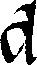
\includegraphics{figures/Bodmer 30_012v_large.jpgstaticd1.png(7, 56, 2)polished.png}}
    \caption{La lettera al termine dell'estrazione.}
    \label{fig:polished_letter}
\end{figure}

\section{Confronto fra lettere}

Questa \`e la fase pi\`u critica dell'intero processo. Si tratta della fase di confronto fra due lettere per vedere se sono la stessa lettera. Visto che \`e una procedura complessa, deve essere suddivisa in procedure pi\`u piccole.

\subsection{Ridimensionamento}\label{ssect:rescaling}

Non \`e scontato (in generale \`e improbabile) che le due lettere che vogliamo confrontare siano delle stesse dimensioni, ma per poterle confrontare vorremmo che lo fossero.

\emph{OpenCV}, cos\`i come molte altre librerie, ci offre una funzione per ridimensionare un'immagine. Quindi un'implementazione banale potrebbe essere quella di ridimensionare una delle immagini per renderla della stessa dimensione dell'altra. Questo, tuttavia comporterebbe una perdita delle proporzioni originali, e quindi non potr\`a andare bene visto che la forma di una lettera cos\`i come la intendiamo dipende strettamente dalle sue proporzioni.

\subsubsection{Metodo centrale}

Un altro metodo semplice, ma sicuramente pi\`u intelligente consiste nell'aggiungere colonne bianche all'immagine pi\`u stretta in quantit\`a uguale a destra e a sinistra e, successivamente, aggiungere righe bianche a quella pi\`u bassa (scelta fra quella che prima era la pi\`u larga e quella ottenuta dall'aggiunta di colonne alla pi\`u stretta), ancora una volta in quantit\`a uguale sopra e sotto. Chiaramente i passaggi possono essere scambiati, ovvero possiamo anche prima le righe e poi le colonne. Inutile dire che se le righe o le colonne da aggiungere sono in numero dispari, si dovr\`a dare una preferenza ad una delle due direzioni, ma se le immagini hanno una risoluzione abbastanza elevata, ci si pu\`o aspettare che questa scelta non porti a differenze sostanziali. Nel corso del testo ci si riferir\`a a questo metodo chiamandolo il metodo centrale o metodo statico, visto che le immagini vengono confrontate allineandone i centri senza spostarli.

\subsubsection{Metodo proporzionale}

Un altro metodo, che in particolari situazioni pu\`o risultare pi\`u efficace, potrebbe essere quello di ridimensionare proporzionalmente l'immagine pi\`u stretta e, in un secondo momento, aggiungere righe bianche a quella pi\`u bassa. Come prima, anche in questo caso possiamo invertire le dimensioni, ovvero ridimensionare la pi\`u bassa e poi aggiungere righe alla pi\`u stretta. Come si pu\`o intuire questo metodo \`e pi\`u efficace quando ci sono lettere di diversa dimensione, ma con lo stesso stile di scrittura, visto che si ha un ridimensionamento proporzionale di una delle lettere.

\subsubsection{Metodo del baricentro}

Si tratta di una variazione al metodo centrale. La differenza sostanziale \`e che con questo metodo, invece di allineare i centri, si allineano i baricentri. Questo comporta che le righe e le colonne vengano aggiunte in due passaggi: si aggiungono prima righe in alto all'immagine che sporge meno verso l'alto, e si aggiungono righe in basso all'immagine che sporge meno verso il basso (che non necessariamente sar\`a la stessa immagine di prima). Verr\`a fatto un procedimento analogo per le colonne, guardando indipendentemente a destra e a sinistra.

Ricordiamo come si calcolano le coordinate del baricentro (o del centro di massa). In ogni immagine associamo un peso pari a 1 ai pixel neri e un peso pari a 0 ai pixel bianchi. Se consideriamo un'immagine $A$ con $m$ righe e $n$ colonne e indichiamo con $A^i_j$ l'elemento di $A$ alla riga $i$-esima e alla colonna $j$-esima, il baricentro si calcola nel modo seguente:

\begin{equation*}
    \left( 
        \frac
            {\displaystyle{\sum_{0 \le i < m} \sum_{0 \le j < n} i A^i_j}}
            {\displaystyle{\sum_{0 \le i < m} \sum_{0 \le j < n} A^i_j}}
        \quad , \quad
        \frac
            {\displaystyle{\sum_{0 \le i < m} \sum_{0 \le j < n} j A^i_j}}
            {\displaystyle{\sum_{0 \le i < m} \sum_{0 \le j < n} A^i_j}}
    \right)
\end{equation*}

Dove la prima coordinata si riferisce alla riga e la seconda alla colonna.

Per semplificare la formula, da ora in avanti daremo per scontato che l'indice $i$ va da 0 a $m$ e l'indice $j$ da 0 a $n$. Adoperando questo abuso di notazione e un'ulteriore semplificazione, possiamo indicare il baricentro come segue.

\begin{equation*}
    \left(
        \frac
            {\displaystyle{\sum_i i \sum_j A^i_j}}
            {\displaystyle{\sum_{i,j} A^i_j}}
        \quad , \quad
        \frac
            {\displaystyle{\sum_j j \sum_i A^i_j}}
            {\displaystyle{\sum_{i,j} A^i_j}}
    \right)
\end{equation*}

Portando fuori il denominatore otteniamo infine:

\begin{equation*}
    \frac{1}{\displaystyle{\sum_{i,j} A^i_j}}
    \left(
        \sum_i i \sum_j A^i_j
        \quad , \quad
        \sum_j j \sum_i A^i_j
    \right)
\end{equation*}

\subsubsection{Metodo del momento di inerzia}

Questo metodo \`e un'evoluzione del metodo del baricentro. Infatti si comporta in maniera simile a questo, ma aggiungendo un passaggio ulteriore. Una volta allineate le immagini con i corrispettivi baricentri, si scala l'immagine con il momento di inerzia minore, in modo che abbiano entrambe lo stesso momento di inerzia. A questo punto si procede come prima per rendere le immagini delle stesse dimensioni.

Prima di mostrare il calcolo del momento di inerzia, definiamo altre notazioni per semplificare le formule.

\begin{equation*}
    s(A) := \sum_{i,j} A^i_j
\end{equation*}

\begin{equation*}
    s^i(A) := \sum_j A^i_j
\end{equation*}

\begin{equation*}
    s_j(A) := \sum_i A^i_j
\end{equation*}

Ora che abbiamo queste tre definizioni possiamo semplificare ulteriormente la formula del baricentro che avevamo trovato in precedenza in questo modo:

\begin{equation*}
    \frac{1}{s(A)}
    \left(
        \sum_i i s^i(A)
        \quad , \quad
        \sum_j j s_j(A)
    \right)
\end{equation*}

Vediamo adesso come calcolare il momento di inerzia. La formula di partenza \`e questa:

\begin{equation*}
    \sum_{i,j} A^i_j \left( (i-\tilde{ \imath })^2 + (j-\tilde{ \jmath })^2 \right)
\end{equation*}

Dove $\tilde{\imath}$ e $\tilde{\jmath}$ sono le coordinate del centro di massa. Il problema con questa formula \`e la sua inefficienza quando usata come algoritmo. Vedremo adesso come renderla pi\`u efficiente per passaggi successivi.

\begin{equation*}
    \left( \sum_{i,j} A^i_j (i-\tilde{ \imath })^2 \right)
    +
    \left( \sum_{i,j} A^i_j (j-\tilde{ \jmath })^2 \right)
\end{equation*}

Concentriamoci adesso solo su uno dei due addendi. I passaggi saranno analoghi per l'altro.

\begin{equation*}
    \sum_i (i-\tilde{ \imath })^2 \sum_j A^i_j
\end{equation*}

\begin{equation*}
    \sum_i (i-\tilde{ \imath })^2 s^i(A)
\end{equation*}

\begin{equation*}
    \sum_i (i^2 - 2i\tilde{\imath} + \tilde{\imath}^2) s^i(A)
\end{equation*}

\begin{equation*}
    \sum_i i^2 s^i(A) - 2 \tilde{\imath} \sum_i i s^i(A) + \tilde{\imath}^2 \sum_i s^i(A)
\end{equation*}

\begin{equation*}
    \sum_i i^2 s^i(A) - 2 \tilde{\imath} \cdot \tilde{\imath} s(A) + \tilde{\imath}^2 s(A)
\end{equation*}

\begin{equation*}
    \sum_i i^2 s^i(A) - \tilde{\imath}^2 s(A)
\end{equation*}

\begin{equation*}
    \sum_i i^2 s^i(A) - \left( \frac{\displaystyle{\sum_i i s^i(A)}}{s(A)} \right)^2 s(A)
\end{equation*}

\begin{equation*}
    \sum_i i^2 s^i(A) - \frac{\displaystyle{\left(\sum_i i s^i(A)\right)}^2}{s(A)}
\end{equation*}

Ricordandoci dell'addendo che avevamo lasciato da parte, il calcolo diventa il seguente:

\begin{equation*}
    \sum_i i^2 s^i(A) + \sum_j j^2 s_j(A)
    - \frac
        {\displaystyle{
            \left(
                \sum_i i s^i(A)
            \right) ^2
            +
            \left(
                \sum_j j s_j(A)
            \right) ^2
        }}
        {s(A)}
\end{equation*}

Nonostante il calcolo appaia pi\`u complicato di quello di partenza, \`e pi\`u semplice sia per un computer che per un umano. La parte complicata prima stava nel trovare il quadrato di un numero reale, adesso dobbiamo fare il quadrato solamente di numeri interi.

Adesso per\`o di quanto devo scalare l'immagine con minor momento di inerzia per fare in modo che abbia lo stesso momento di inerzia dell'altra? Per rispondere a questa domanda devo guardare la formula del momento di inerzia e rendermi conto che le $i$ e le $j$ (che in fisica corrispondono con le lunghezze) appaiano con un esponente quadratico. Quindi, se si scala l'immagine di un fattore $r$ (ovvero si moltiplicano le $i$ e le $j$ per $r$ e se ne sommano $r$ volte tante), ottengo la stessa cosa che se si fosse moltiplicata l'espressione per $r^4$.

La conclusione \`e che devo scalare l'immagine di un fattore pari a:

\begin{equation*}
    r = \sqrt[4]{\frac{I_1}{I_2}}
\end{equation*}

Dove $I_1$ e $I_2$ sono i momenti di inerzia delle due immagini di partenza.

\subsection{Indice di Jaccard}\label{ssect:jaccard}

Una volta che le due lettere hanno le stesse dimensioni, possiamo usare l'indice di Jaccard per confrontarle.

L'indice di Jaccard \`e un indice che possiamo utilizzare per misurare la somiglianza fra due insiemi. Dati due insiemi $A$ e $B$, l'indice di Jaccard si calcola come:

\begin{equation*}
    \frac{\vert A \cap B \vert}{\vert A \cup B \vert}
\end{equation*}

In questo caso l'insieme associato a ciascuna immagine comprende le posizioni dei pixel neri. Dunque l'indice rappresenta il rapporto fra il numero di pixel che sono neri in entrambe le immagini e il numero di pixel che sono neri in almeno una immagine.

Per avere una visione di come l'indice di Jaccard confronta due lettere possiamo guardare la figura \ref{fig:Jaccard}. In tale figura si pu\`o vedere il confronto fra le lettere a sinistra. L'area occupata dalla sola lettera di figura di sinistra \`e colorata in giallo, quella occupata dalla sola lettera di figura di destra \`e colorata in blu e quella occupata da entrambe le lettere \`e verde. In questo caso l'indice di Jaccard risulta essere circa $0.53$.

\begin{figure}
    \centering
    \begin{tabular}{c c c}
        \begin{minipage}{.3\textwidth}
        \centering
        \frame{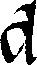
\includegraphics[]{figures/Bodmer 30_012v_large.jpgstaticd1.png(7, 56, 2)polished.png}}
        \end{minipage}
         & 
        \begin{minipage}{.3\textwidth}
        \centering
        \frame{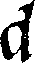
\includegraphics[]{figures/Bodmer 30_012v_large.jpgstaticd1.png(8, 72, 2).png}}
        \end{minipage}
         & 
        \begin{minipage}{.3\textwidth}
        \centering
        \frame{
\includegraphics[]{figures/Bodmer 30_012v_large.jpgstaticd1.png(8, 72, 2)_jaccard_0.534452296819788.png}}
        \end{minipage}
    \end{tabular}
    \caption{In nero due lettere e a destra la rappresentazione del loro indice di Jaccard. In giallo la prima lettera, in blu la seconda e  in verde la loro intersezione.}
    \label{fig:Jaccard}
\end{figure}

Se si utilizzano immagini scelte appositamente, come quelle di figura \ref{fig:visual_test_input}, si riesce a capire bene quali sono le differenze fra i vari metodi descritti nella sezione \ref{ssect:rescaling}. In figura \ref{fig:visual_jaccard_test} si pu\`o apprezzare intuitivamente come funzionano i tre metodi. Si vede infatti che il metodo centrale allinea i centri delle immagini (in questo caso gli angoli dei quadrati), il metodo del baricentro allinea i baricentri (i centri dei quadrati), e il metodo inerziale, oltre ad allineare i baricentri, scala l'immagine pi\`u piccola in modo da avere lo stesso momento di inerzia della pi\`u grande (in questo esempio in modo che i quadrati abbiano le stesse dimensioni).

\begin{figure}
    \centering
    \begin{tabular}{c c}
        \begin{minipage}{.3\textwidth}
            \centering
            \frame{
\includegraphics{figures/visual-test-input-0.png}}
        \end{minipage}
        &
        \begin{minipage}{.3\textwidth}
            \centering
            \frame{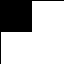
\includegraphics{figures/visual-test-input-1.png}}
        \end{minipage}
    \end{tabular}
    \caption{Le due immagini usare come test. Da notare che il bordo fine non fa parte dell'immagine.}
    \label{fig:visual_test_input}
\end{figure}

\begin{figure}
    \centering
    \begin{tabular}{c c c}
        \begin{minipage}{.3\textwidth}
            \centering
            \frame{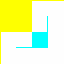
\includegraphics{figures/visual-test-0.png}}
        \end{minipage}
        &
        \begin{minipage}{.3\textwidth}
            \centering
            \frame{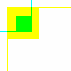
\includegraphics{figures/visual-test-1.png}}
        \end{minipage}
        &
        \begin{minipage}{.3\textwidth}
            \centering
            \frame{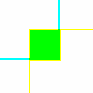
\includegraphics{figures/visual-test-2.png}}
        \end{minipage}
    \end{tabular}
    \caption{Le due immagini di test sovrapposte utilizzando le tre modalit\`a. A sinistra il metodo centrale, nel mezzo il metodo del baricentro, e a destra il metodo inerziale.}
    \label{fig:visual_jaccard_test}
\end{figure}